\chapter{Конструкторский раздел}
В конструкторской части разработано программное обеспечение, а также формально описаны применяемые алгоритмы.

\section{Описание структур данных}
!!!!
\section{Общий алгоритм }
\section{Схемы алгоритм визуализации трехмерной схемы}
\subsection{Алгоритм z-буффер}
На рисунке~\ref{fig:cloud_fcc} представлена схема алгоритма z-буфера.
\begin{figure}[H]
	\centering
	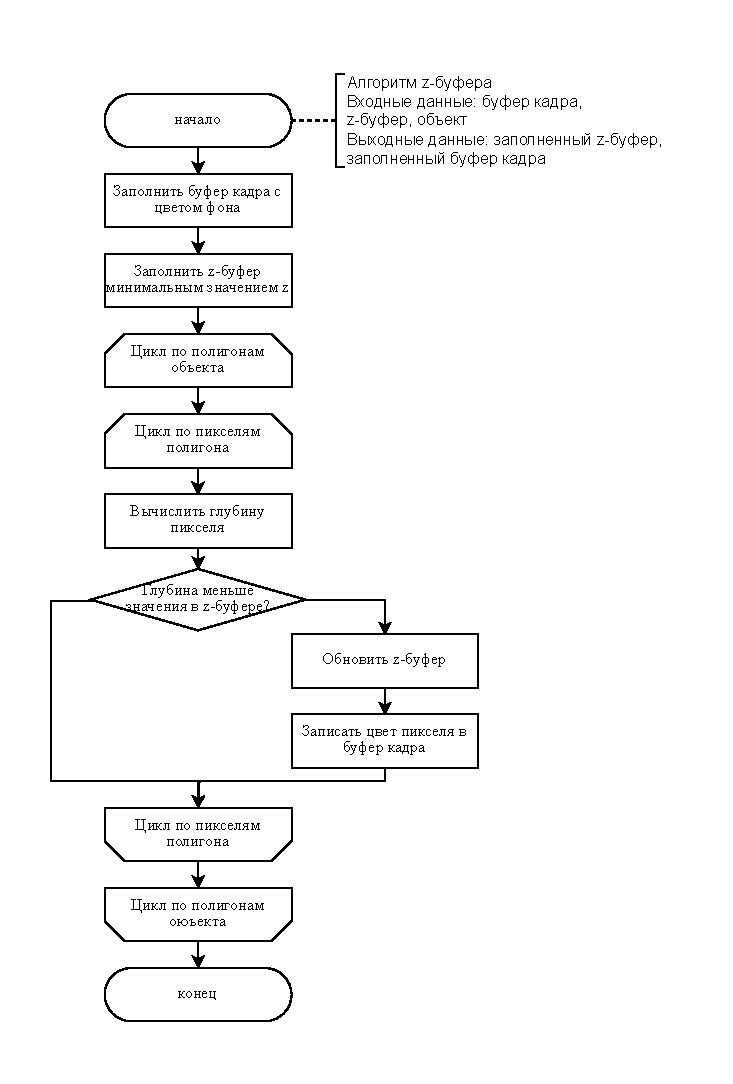
\includegraphics[width=1.0\textwidth, page=1]{assets/img/z_buf_alg.pdf}   
	\caption{Схема алгоритма z-буфера}
	\label{fig:cloud_fcc}
\end{figure}

На рисунке~\ref{fig:cloud_fc1} представлена схема алгоритма z-буфера.
\begin{figure}[H]
	\centering
	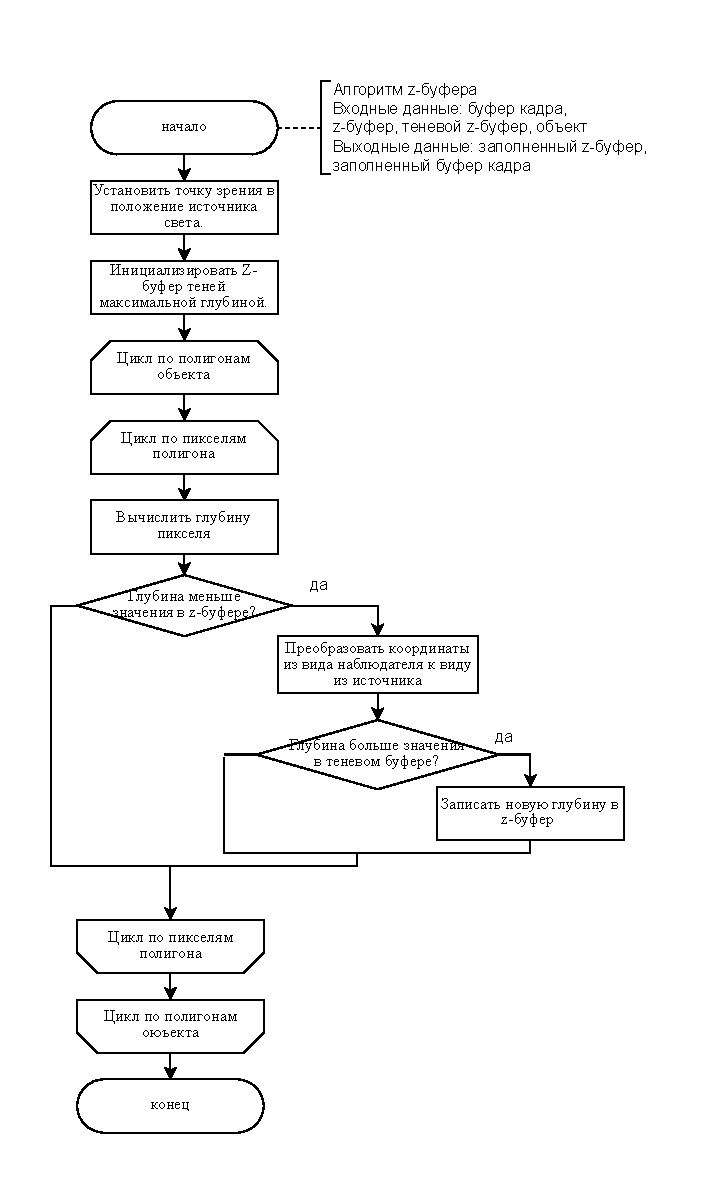
\includegraphics[width=0.8\textwidth, page=1]{assets/img/z_buf_shadow_alg.pdf}   
	\caption{Схема алгоритма алгоритма теневого z-буфера}
	\label{fig:cloud_fc1}
\end{figure}

На рисунке~\ref{fig:cloud_fc2} представлена схема алгоритма имитации ветра.
\begin{figure}[H]
	\centering
	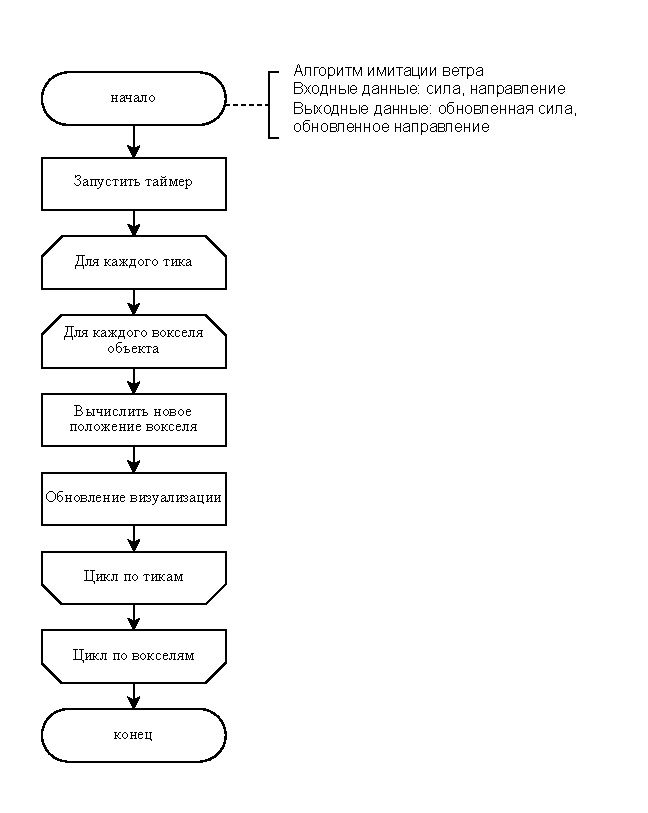
\includegraphics[width=1.0\textwidth, page=1]{assets/img/wind_alg.pdf}   
	\caption{Схема алгоритма имитации ветра.}
	\label{fig:cloud_fc2}
\end{figure}

\section*{Вывод}
В разделе спроектировано разрабатываемое программное обеспечение для визуализации сакуры, качающейся на ветру, приведены схемы алгоритмов.
